% Be sure to write chapter titles in ALL CAPS
\chapter{\uppercase{BACKGROUND}}

This chapter is divided into four sections. First, I provide some background on the Tor anonymity network and describe how clients can contact hidden services inside it. As a background for Namecoin, I secondly explain Bitcoin and its architecture. Third, I provide background on Namecoin and compare and contrast with Bitcoin. Finally, I provide an overview of traditional DNS and how it is used on the clearnet.



\section{Tor}

The Tor network is a second-generation onion routing system that aims to provide anonymity, privacy, and Internet censorship protection to its users. Tor routes encrypted TCP/IP traffic through a worldwide volunteer-run network of over six thousand relays. Tor's encryption, authentication, and routing protocols are designed to make it infeasible for any adversary to identify an end user or reveal their traffic. Despite attempts by agencies and governments to block, tap, or crack the Tor network, Tor remains one of the most popular and secure tools to use against network surveillance, traffic analysis, and information censorship.

\subsection{Design}

Tor provides an anonymity and privacy layer by relaying all end-user TCP traffic through a series of relays on the Tor network. Typically this route consists of a carefully-constructed three-hop path known as a \textit{circuit}, which changes over time. These nodes in the circuit are commonly referred to as \textit{guard node}, \textit{middle relay}, and the \textit{exit node}, respectively. Only the first node can determine the origin of TCP traffic into Tor, and only the exit node can see the destination of traffic out of Tor. The middle router is unable to determine either. Furthermore, each node is only aware of the machines it talks to, so only the client knows the identity of all three nodes used in its circuit. Tor's architecture is designed to make it exceptionally difficult for a well-resourced adversary to uncover the identity of the end-user and their network activities, even if nodes are compromised.\cite{McCoy2008}

\subsection{Routing}

In traditional Internet connections, the client communicates directly with the server. In this model, an eavesdropper can often reveal both the identity of the end user and their activities. Direct encrypted connections do not hide IP headers, which expose source and destination addresses and the size of the payload. In the face of adversaries with sophisticated traffic analysis tools, such information can be very revealing for someone who wishes to hide their activities altogether.

Tor combats this by routing end user traffic through a randomized circuit through the network of relays. The Tor client software first queries a trusted directory server or a relay mirroring the directory. This directory contains of list of IPs, ports, public keys, and other information about all nodes in the Tor network.\cite{Xin2009} Next, the Tor client chooses three unique and geographically diverse nodes to use. It then builds and extends the circuit one node at at time, negotiating respective HTTPS connections with each node in turn. No single relay knows the complete path, and each relay can only decrypt its layer of decryption. In this way, data is encrypted multiple times and then is decrypted in an onion-like fashion as it passes through the circuit.

\begin{figure}[htdp]
	\begin{minipage}[b]{0.45\linewidth}
		\centering
		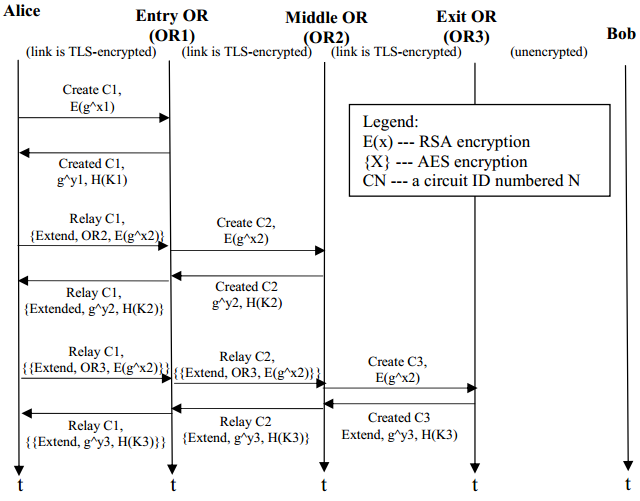
\includegraphics[width=\textwidth]{images/circuit-construction.png}
		\caption{Anatomy of the construction of a Tor circuit.}
		\label{fig:figure1}
	\end{minipage}
	\hspace{0.5cm}
	\begin{minipage}[b]{0.45\linewidth}
		\centering
		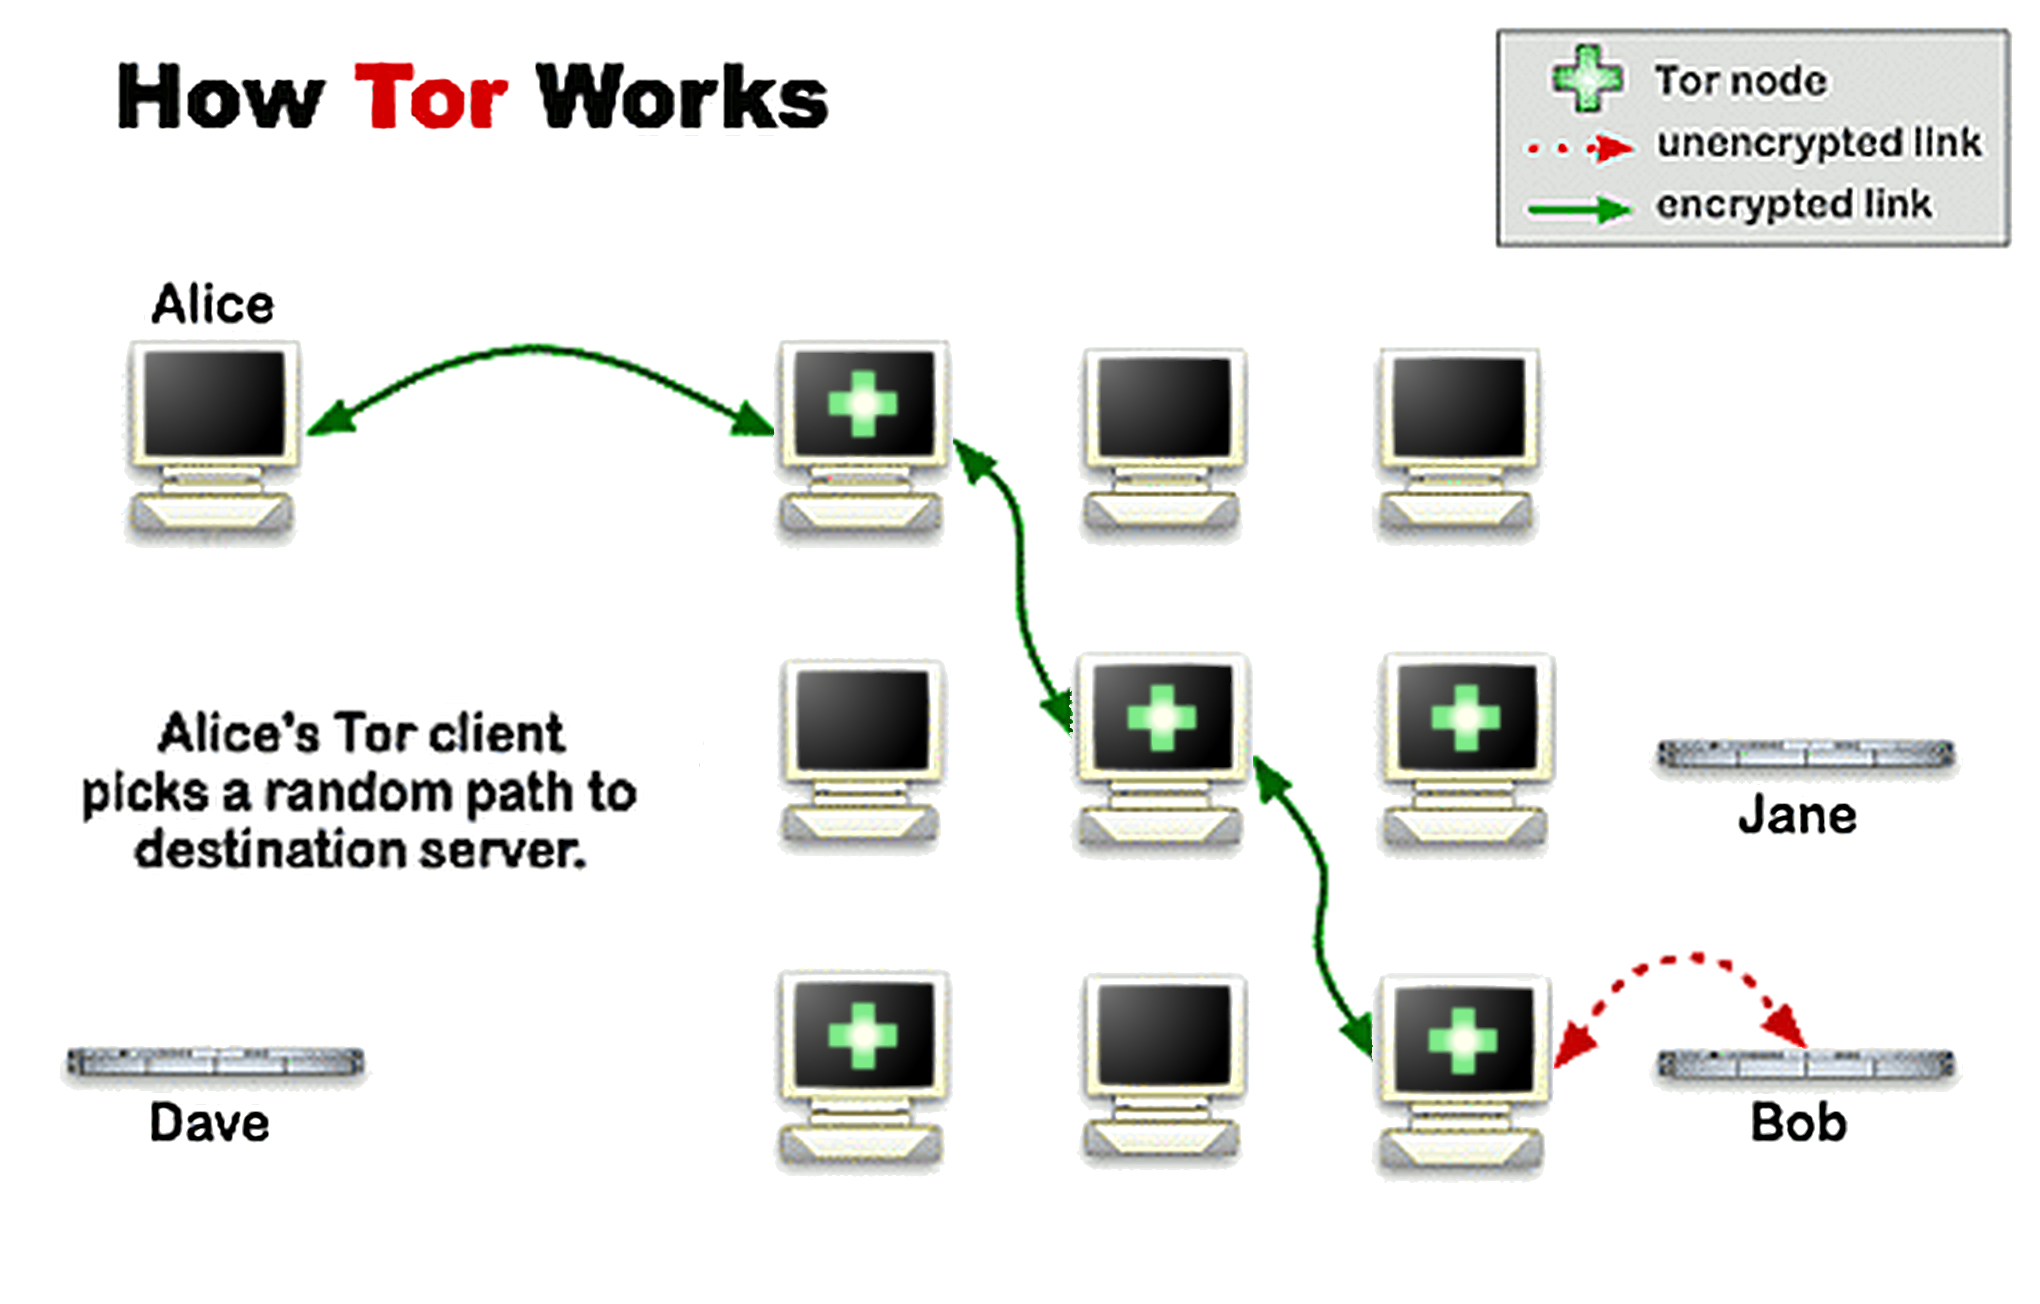
\includegraphics[width=\textwidth]{images/circuit-building-2-5.png}
		\caption{A circuit through the Tor network.}
		\label{fig:figure2}
	\end{minipage}
\end{figure}

The client first establishes a TLS connection with the first relay, $R_{1}$, using the relay's public key. The client then performs a Diffie-Hellman-Merkle key exchange to negotiate $K_{1}$ which is then used to generate two symmetric session keys: a forward key $K_{1,F}$ and a backwards key $K_{1,B}$. $K_{1,F}$ is used to encrypt all communication from the client to $R_{1}$ and $K_{1,B}$ is used for all replies from $R_{1}$ to the client. These keys are used conjunction with the symmetric cipher suite negotiated during the TLS handshake, thus forming an encrypted tunnel with perfect forward secrecy. Once this one-hop circuit has been created, the client then sends $R_{1}$ the RELAY\_EXTEND command, the address of $R_{2}$, and the client's half of the Diffie-Hellman-Merkle protocol ($ g^a mod b $) using $K_{1,F}$. $R_{1}$ performs a TLS handshake with R${2}$ and uses $R_{2}$'s public key to send $ g^a mod b $ to $R_{2}$, who replies with his half of the handshake and a hash of $K_{2}$. $R_{1}$ then forwards this to the client under $R_{1,B}$ with the RELAY\_EXTENDED command to notify the client. The client generates $K_{1,F}$ and $K_{1,B}$ from $K_{2}$, and repeats the process for $R_{3}$,\cite{Ling2012} as shown in Figure 3. The TLS/IP connections remain open, so the returned information travels back up the circuit to the end user.

Following the complete establishment of a circuit, the Tor client software then offers a Secure Sockets (SOCKS) interface on localhost which multiplexes TCP traffic through Tor. At the application layer, this data is packed and padded into equally-sized Tor \textit{cells}, transmission units of 512 bytes. As each relay sees no more than one hop in the circuit, in theory neither an eavesdropper nor a compromised relay can link the connection's source, destination, and content. Tor further obfuscates user traffic by changing the circuit path every ten minutes,\cite{McCoy2008} as shown in Figure 4. A new circuit can also be requested manually by the user.

\begin{figure}[htbp]
	\centering
	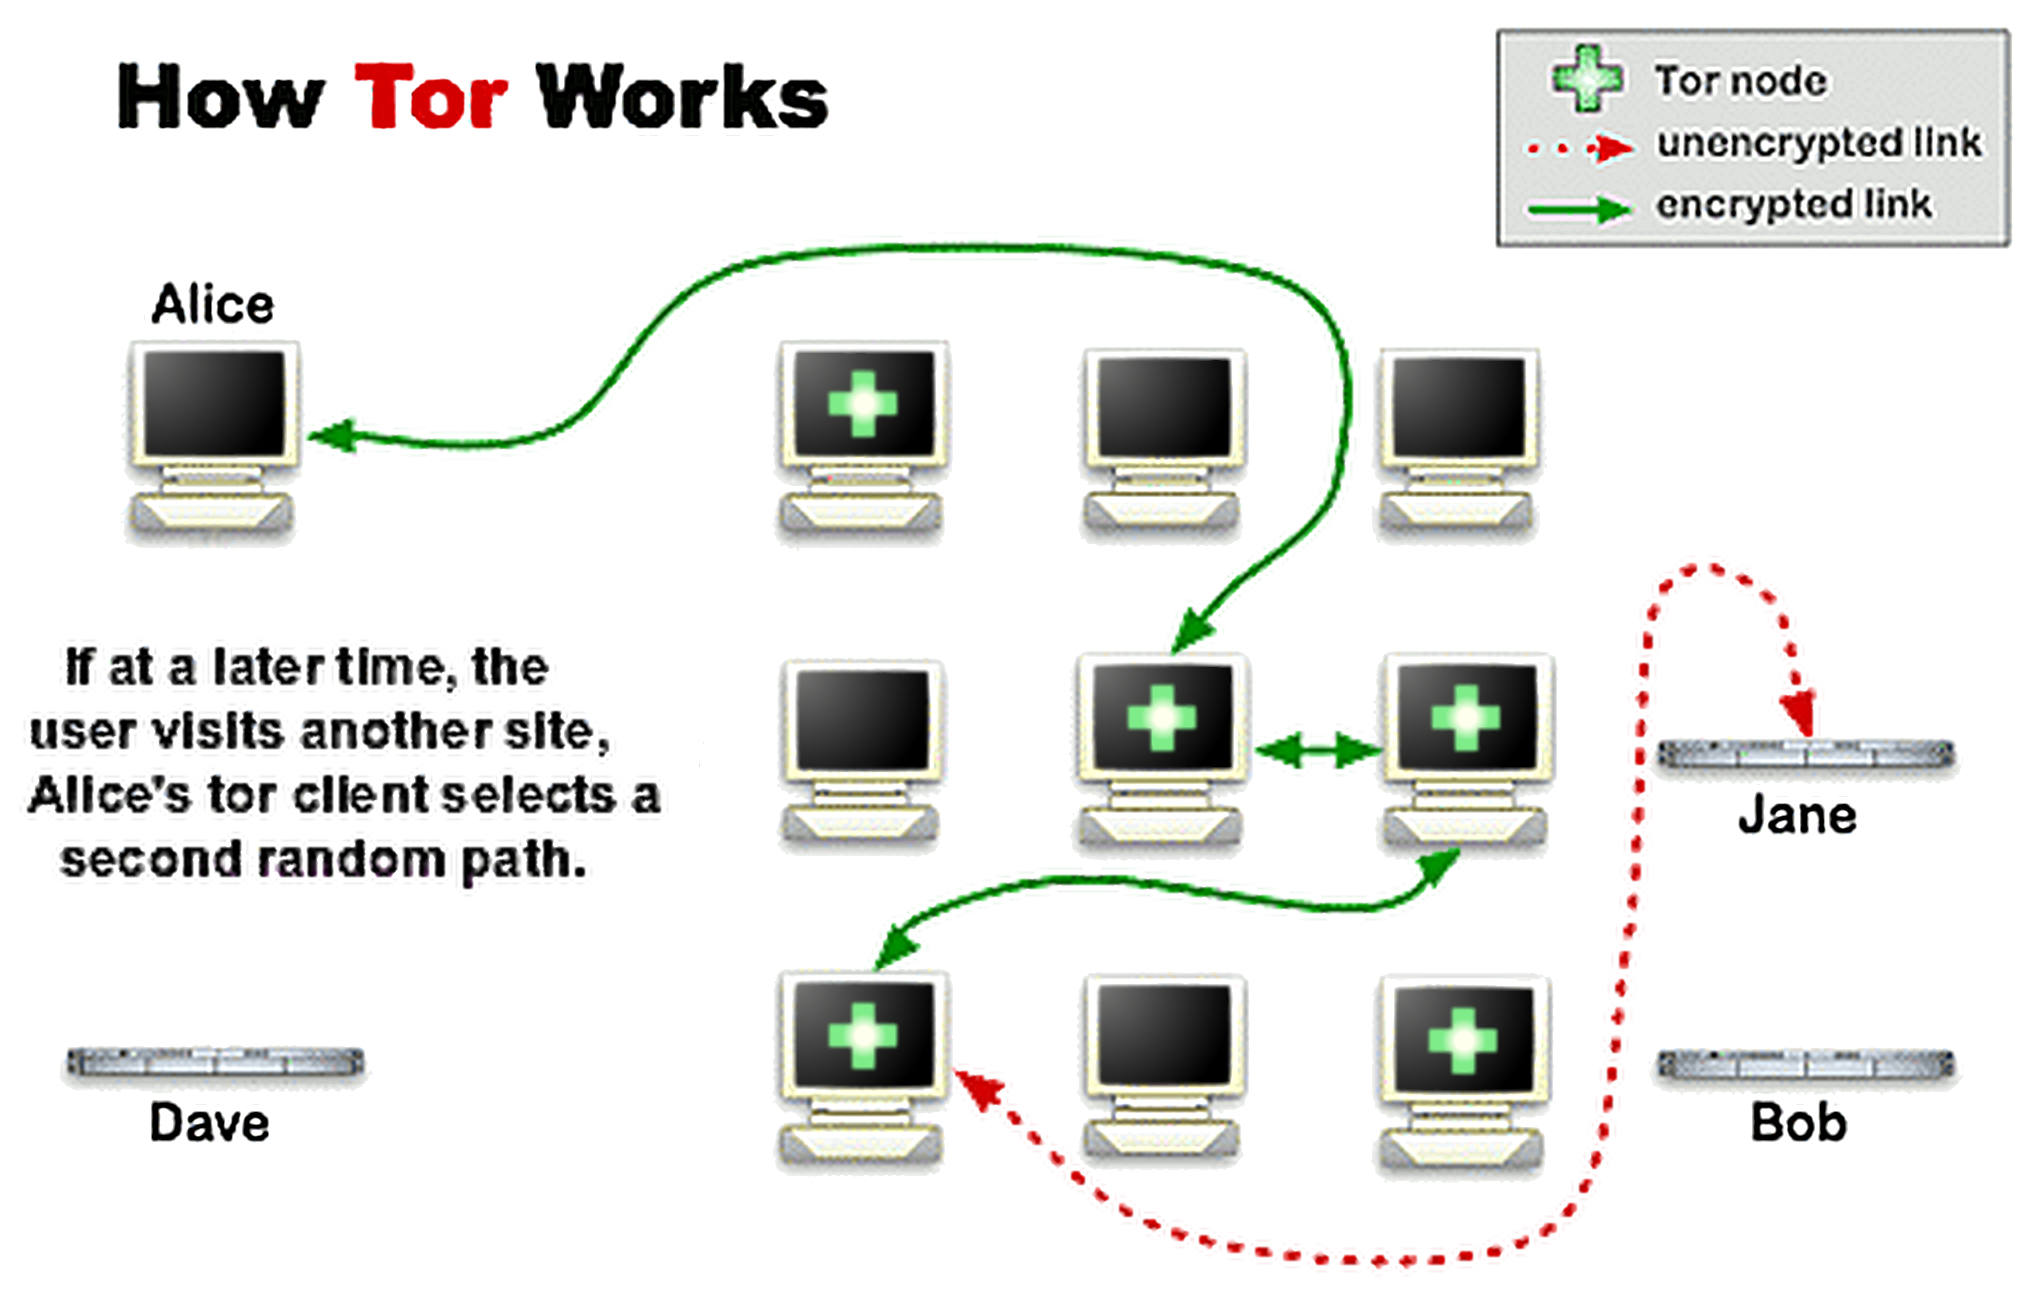
\includegraphics[width=0.6\textwidth]{images/circuit-change-1-4.png}
	\caption{A Tor circuit is changed periodically, creating a new user identity.}
	\label{fig:figure1}
\end{figure}

% Although a different guard node is used here, in practice the choice of entry point is preserved for extended periods of time.

An encrypted connection is often established with the other client or web server, depending on whether or not the recipient supports encryption. If this is the case, even the exit node cannot see the traffic in cleartext. An outsider is therefore faced with up to four layers of TLS encryption: $K_{1,F}(K_{2,F}(K_{3,F}(K_{server}(client\ request))))$ and likewise $K_{1,B}(K_{2,B}(K_{3,B}(K_{server}(server\ reply))))$ for the returning traffic. This makes traffic analysis and cryptographic attacks very difficult.

Tor users typically use the Tor Browser Bundle, (TBB) a custom build of Mozilla Firefox with a focus on security and privacy. The TBB anonymizes and provides privacy to the user in many ways. These include blocking all scripts not explicitly whitelisted, forcing all traffic through the Tor SOCKS port, mimicking Firefox in Windows both with a user agent (regardless of the native platform) and SSL cipher suites, and reducing Javascript timer precision to avoid identification through clock skew. Furthermore, the TBB includes the Electronic Frontier Foundation's HTTPS Everywhere extension, which uses regular expressions to rewrite HTTP web requests into HTTPS whenever possible. Thus, if the web server is capable of handling SSL or TLS connections, HTTP communications will be encrypted to them. If this is the case, the TBB performs a TLS handshake with the web server, but the exchange happens through the Tor circuit. This provides the final layer of encryption to the outside.

\subsection{Hidden Services}

While the majority of Tor's usage is for traditional access to the Internet, Tor's routing scheme also supports anonymous services, such as websites or chatrooms. These are a part of the Deep Web and cannot be normally contacted outside of Tor. Unlike the Clearnet, Tor does not contain a traditional DNS system for its websites; instead, every hidden service has a public and private RSA key, and domains are a truncated SHA-1 hash of its public key. This means that domain names are distributed and correlate directly to the identity of a hidden service, allowing anyone to verify the authenticity of the service server, akin to SSL certificates on the Clearnet. Tor hidden services allow a client, Alice, and a hidden service, Bob, to communicate anonymously.\cite{TorOverview}

In advance, Bob builds Tor circuits to several random relays and enables them to act as \textit{introduction points} by giving them his public key, $B_{K}$. He then uploads this information to a distributed hashtable inside the Tor network, signing the result. Alice queries this hashtable, finds $B_{K}$ and his introduction points, and builds a Tor circuit to one of them, $IP_{1}$. Simultaneously, she also builds a circuit to another relay, $RP$, which she enables as a rendezvous point by telling it a one-time secret, $S$.

\begin{figure}[htdp]
	\begin{minipage}[b]{0.45\linewidth}
		\centering
		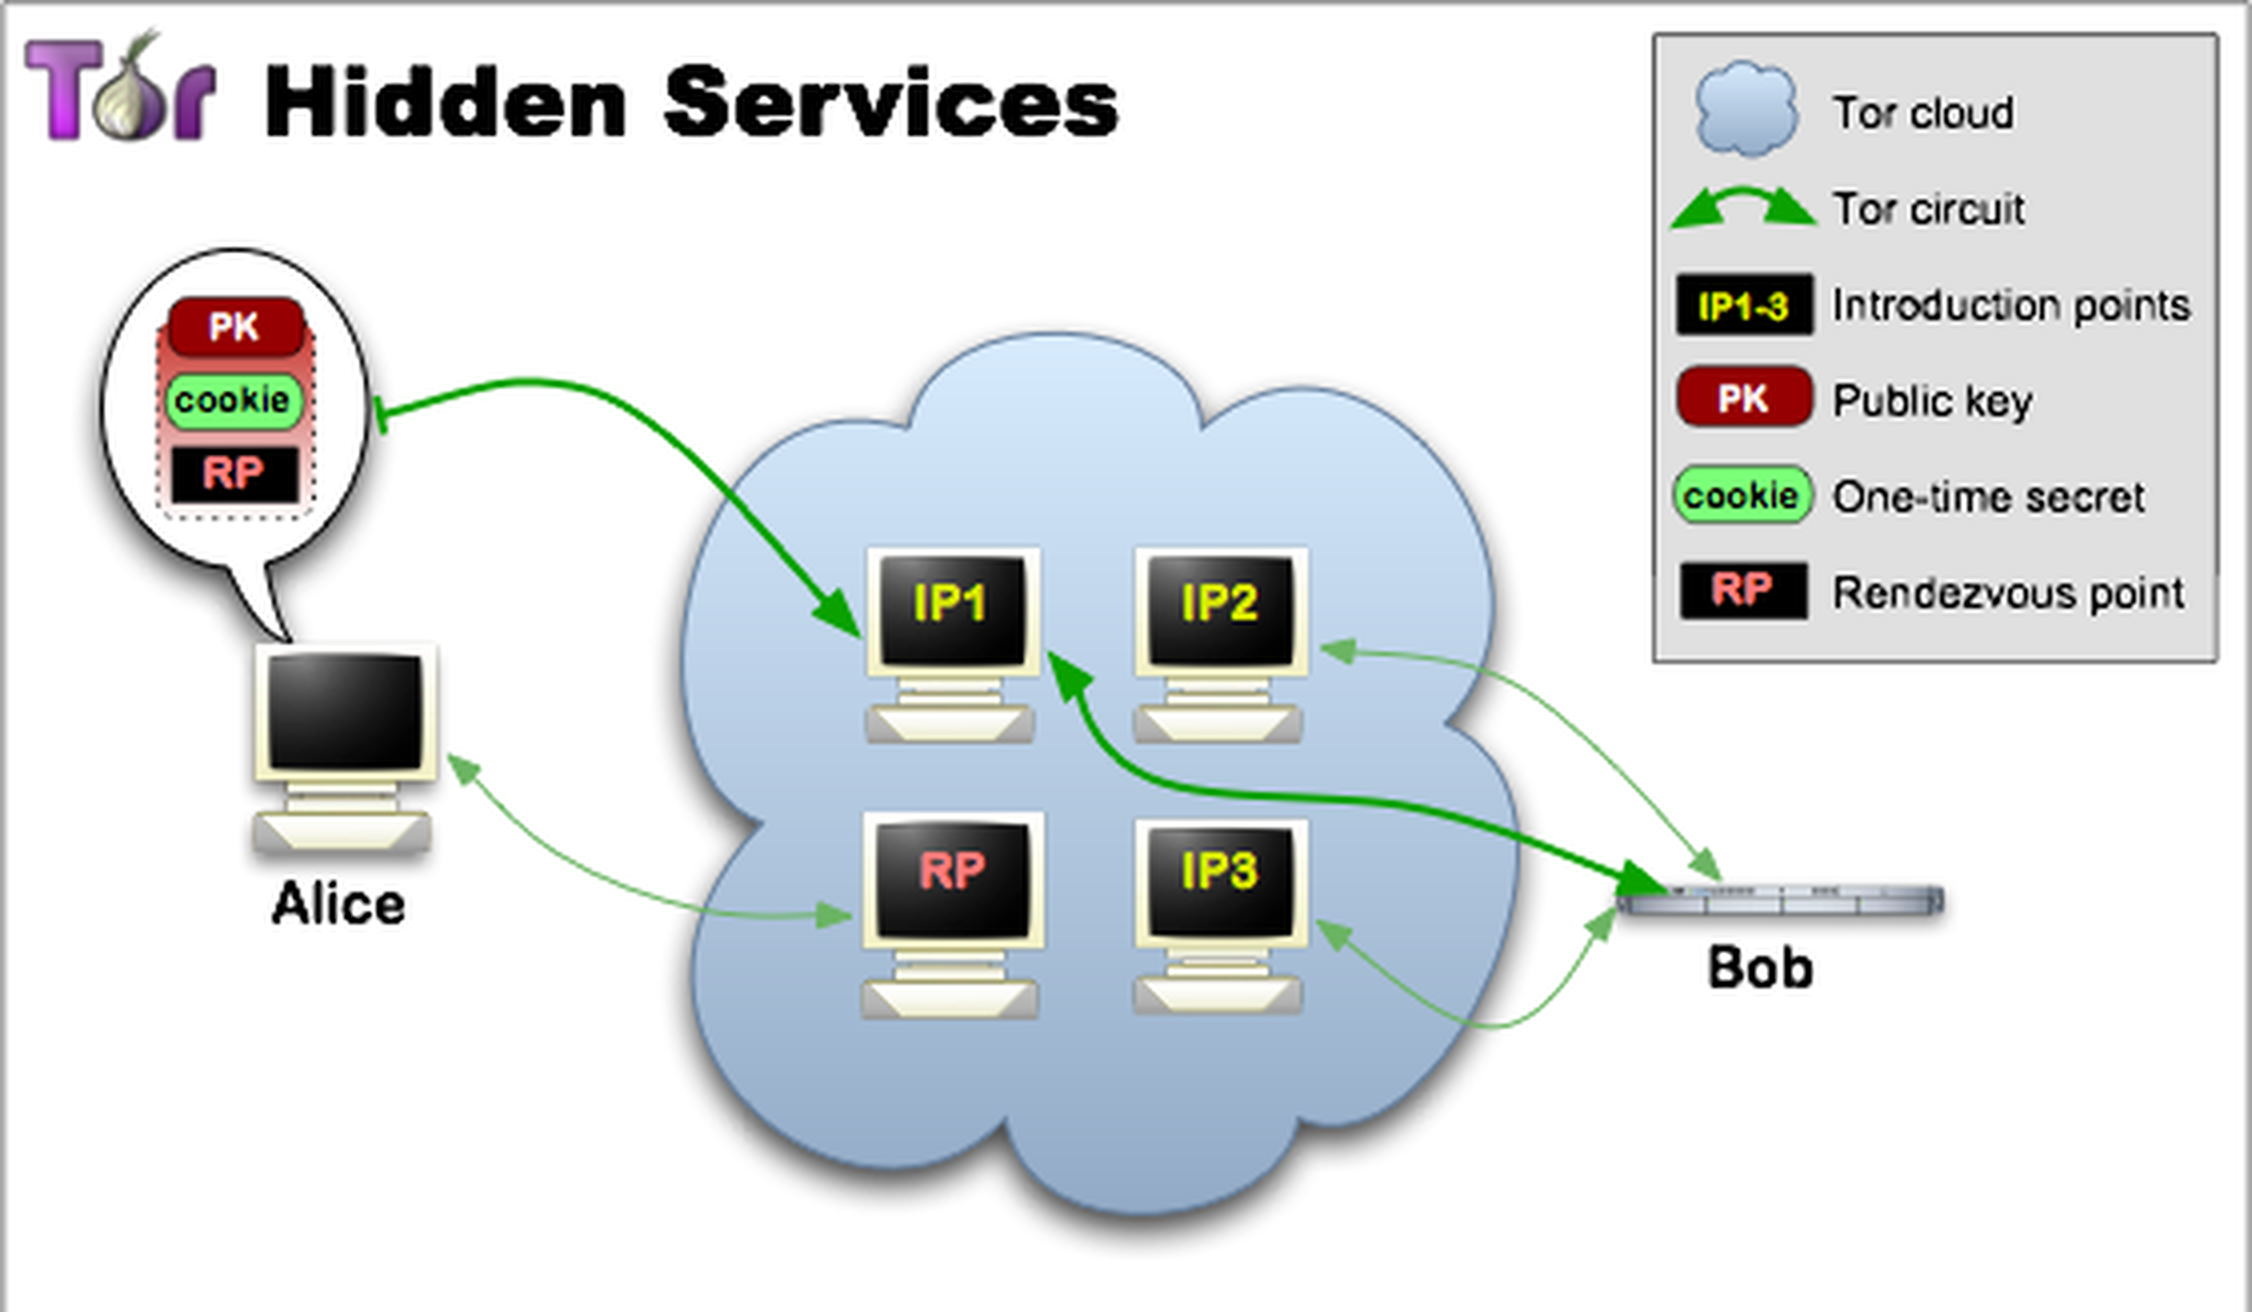
\includegraphics[width=\textwidth]{images/tor-hidden-service-4-higher.png}
		\caption{Alice uses the encrypted cookie to tell Bob to switch to $RP$.}
		\label{fig:figure1}
	\end{minipage}
	\hspace{0.5cm}
	\begin{minipage}[b]{0.45\linewidth}
		\centering
		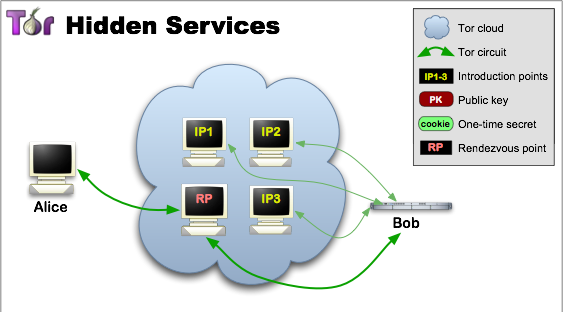
\includegraphics[width=\textwidth]{images/tor-hidden-service-6.png}
		\caption{Bidirectional communication between Alice and the hidden service.}
		\label{fig:figure2}
	\end{minipage}
\end{figure}

She then sends to $IP_{1}$ an cookie encrypted with $B_{K}$, containing $RP$ and $S$. Bob decrypts this message, builds a circuit to $RP$, and tells it $S_{1}$, enabling Alice and Bob to communicate.

%The communication travels through six Tor nodes: three established by Alice and three by Bob.




% TODO: expand: I spend six pages on Tor + hidden services, I should spend six pages on BTC + Namecoin, and two on DNS
% question: I'm aiming for 50 pages, and it looks I'll be burning 14 or 15 on introductions. Is that all right? If not, reduce to 5 + 5 + 1
\section{Bitcoin} 

Bitcoin is a decentralized digital cryptocurrency, created by pseudonymous developer Satoshi Nakamoto in 2008. Ownership of Bitcoins consists of holding a private ECDSA key, and a transfer is simply a transmission of Bitcoins from one key to another. All transactions are recorded on a public ledger, called a blockchain, a data structure whose integrity is verified through computational power. Bitcoins are generated computationally at a fixed rate by \textit{miners}, who also secure the blockchain. Although Bitcoin received limited attention in the first two years of its life, it has since grown significantly since then, with approximately 70,000 daily transactions as of the time of this writing. Bitcoin's growth has led to the creation of many alternative cryptocurrencies, and its popularity has influenced financial discussions, legal controversy, and the prices of electronics worldwide.

\subsection{Architecture}

A blockchain is data structure fundamental to Bitcoin, and crucial for its functionality. As a distributed decentralized system, this public ledger is Nakamoto's answer to ensuring agreement of fundamental data across all involved parties. The blockchain is a novel structure, and its structure guarantees integrity, chronological ordering of transactions, and prevention of double-spending of Bitcoins. The blockchain consists of blocks of data that are held together by proof-of-work, a cryptographic puzzle whose solution is provably hard to find but trivial to verify. Bitcoin's proof-of-work is based on Adam Back's Hashcash scheme: that is, find a nonce such that the hash of this nonce meets a certain requirement. In Bitcoin's case this is stated as finding a nonce that when passed through two rounds of SHA-256 ($ \textrm{SHA}256^{{2}} $) produces a value less than or equal to a target $ T $. This requires a party to perform on average $ \frac{1}{Pr[H \leq T]} = \frac{2 ^ {{256}}}{T} $ amount of computations, but it is easy to verify that $ \textrm{SHA}256^{{2}}(\textrm{msg} || n) \leq T $. Nodes in the Bitcoin network collectively agree to use the blockchain with the highest accumulation of computational effort, so an adversary seeking to modify the structure would need to recompute the proof-of-work for all previous blocks as well as out-perform the network, which is infeasible.\cite{Okupski2014}

Each block in the blockchain consists of a header and a payload. The header contains a hash of the previous block's header, the root hash of the Merkle tree built from the transactions in this block, a timestamp, a target $ T $, and a nonce. The target $ T $ changes in response to speed at which the proof-of-work was solved such that blocks are added to the blockchain at a relatively fixed rate. The block payload consists of a list of transactions. The root node of the Merkle tree ensures the integrity of the transaction vector: verifying that a given transaction is contained in the tree takes $ log(n) $ hashes, and a Merkle tree can be built $ n * log(n) $ time, ensuring that all transactions are accounted for. The hash of the previous block in the header ensures that blocks are ordered chronologically, and the Merkle root hash ensures that the transactions contained in each block are order chronologically as well. The $ \textrm{SHA}256^{{2}} $ proof-of-work provides integrity of the data structure, and secp256k1 ECDSA key are used to prove ownership of coins.\cite{Okupski2014}

\begin{figure}[htbp]
	\centering
	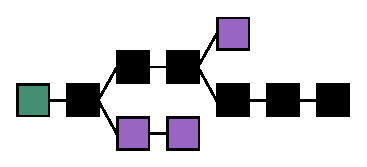
\includegraphics[width=0.6\textwidth]{images/Blockchain-2.eps}
	\caption{A sample blockchain.}
	\label{fig:figure1}
\end{figure}

% In the possibility that multiple nodes solve the proof-of-work and generate a new block simultaneously, the block becomes orphaned, the transactions recycled, and the blockchain follows the longest path from the genesis node to the latest block.

\begin{figure}[htbp]
	\centering
	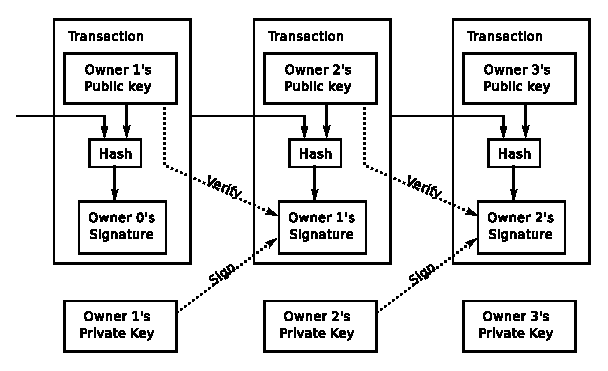
\includegraphics[width=0.6\textwidth]{images/bitcoin_transaction.eps}
	\caption{Three traditional Bitcoin transactions.}
	\label{fig:figure1}
\end{figure}

%Each transaction contains the public  of the recipient, the ECDSA digital signature of the transaction from the sender, and the hash of the originating transaction. In practice transactions can contain multiple input and outputs.

In this way, the digital signatures and proof-of-work in the blockchain can be tracked forwards indefinitely. 






\section{Namecoin}




\section{DNS}

\subsection{Introduction}

\subsection{Architecture}